\section{Performance Evaluation}
\label{sec:evaluation}
In this section, we evaluate the performance of the proposed low-complexity solution framework by numerical simulations.
The experiment setup and compared benchmarks are elaborated in section \ref{subsec:basic}.
The evaluation results are displayed in \ref{subsec:advance}, where some metrics (average cost, average JCT, average throughput) are adopted to prove the performance of our proposed solution framework.
The sensitivity study on parameters is also applied to provide some insights on the robustness of the framework.

\subsection{Experiment Setup}
\label{subsec:basic}
\textbf{Parameters Setup:}
In the simulation, we implement the system in a small scale setting where fully-accessible APs and edge servers are considered.
specifically, there are $K=5$ APs, $M=3$ edge servers, and $J=5$ type of jobs in the system corresponding to the manipulated data trace.
Each time slot is taken as $\tau = 0.05$ i.e. 50ms, and the broadcast interval is taken as $20$ time slots, i.e. $1$ second.
The maximum uploading time is set as $3$ times the broadcast interval, i.e. $\Xi = 3T$.
\fixit{
    The computation time of each job type at each edge server follows the uniform distribution.
}
The distributions of arrival rate, uploading time and processing time are generated randomly.
Each queue for VMs on edge server is set with maximum queue length $L_{max}=20$, i.e. there would be at most $100$ jobs on one edge server.
\fixit{
    We set small maximum queue length, in case to show that how job rejection affects the system.
    % The arrival rate is taken as small probability with enough APs in the system, and correspondingly enough edge servers for the processing.
    % Each queue on edge server with maximum 20 jobs because our algorithm is strong enough to predict the overflow to ensure a reliable system.
}

%-----------------------------------------------------------------------------------------------%
\begin{figure*}[ht!]                                                                            %
    \centering                                                                                  %
    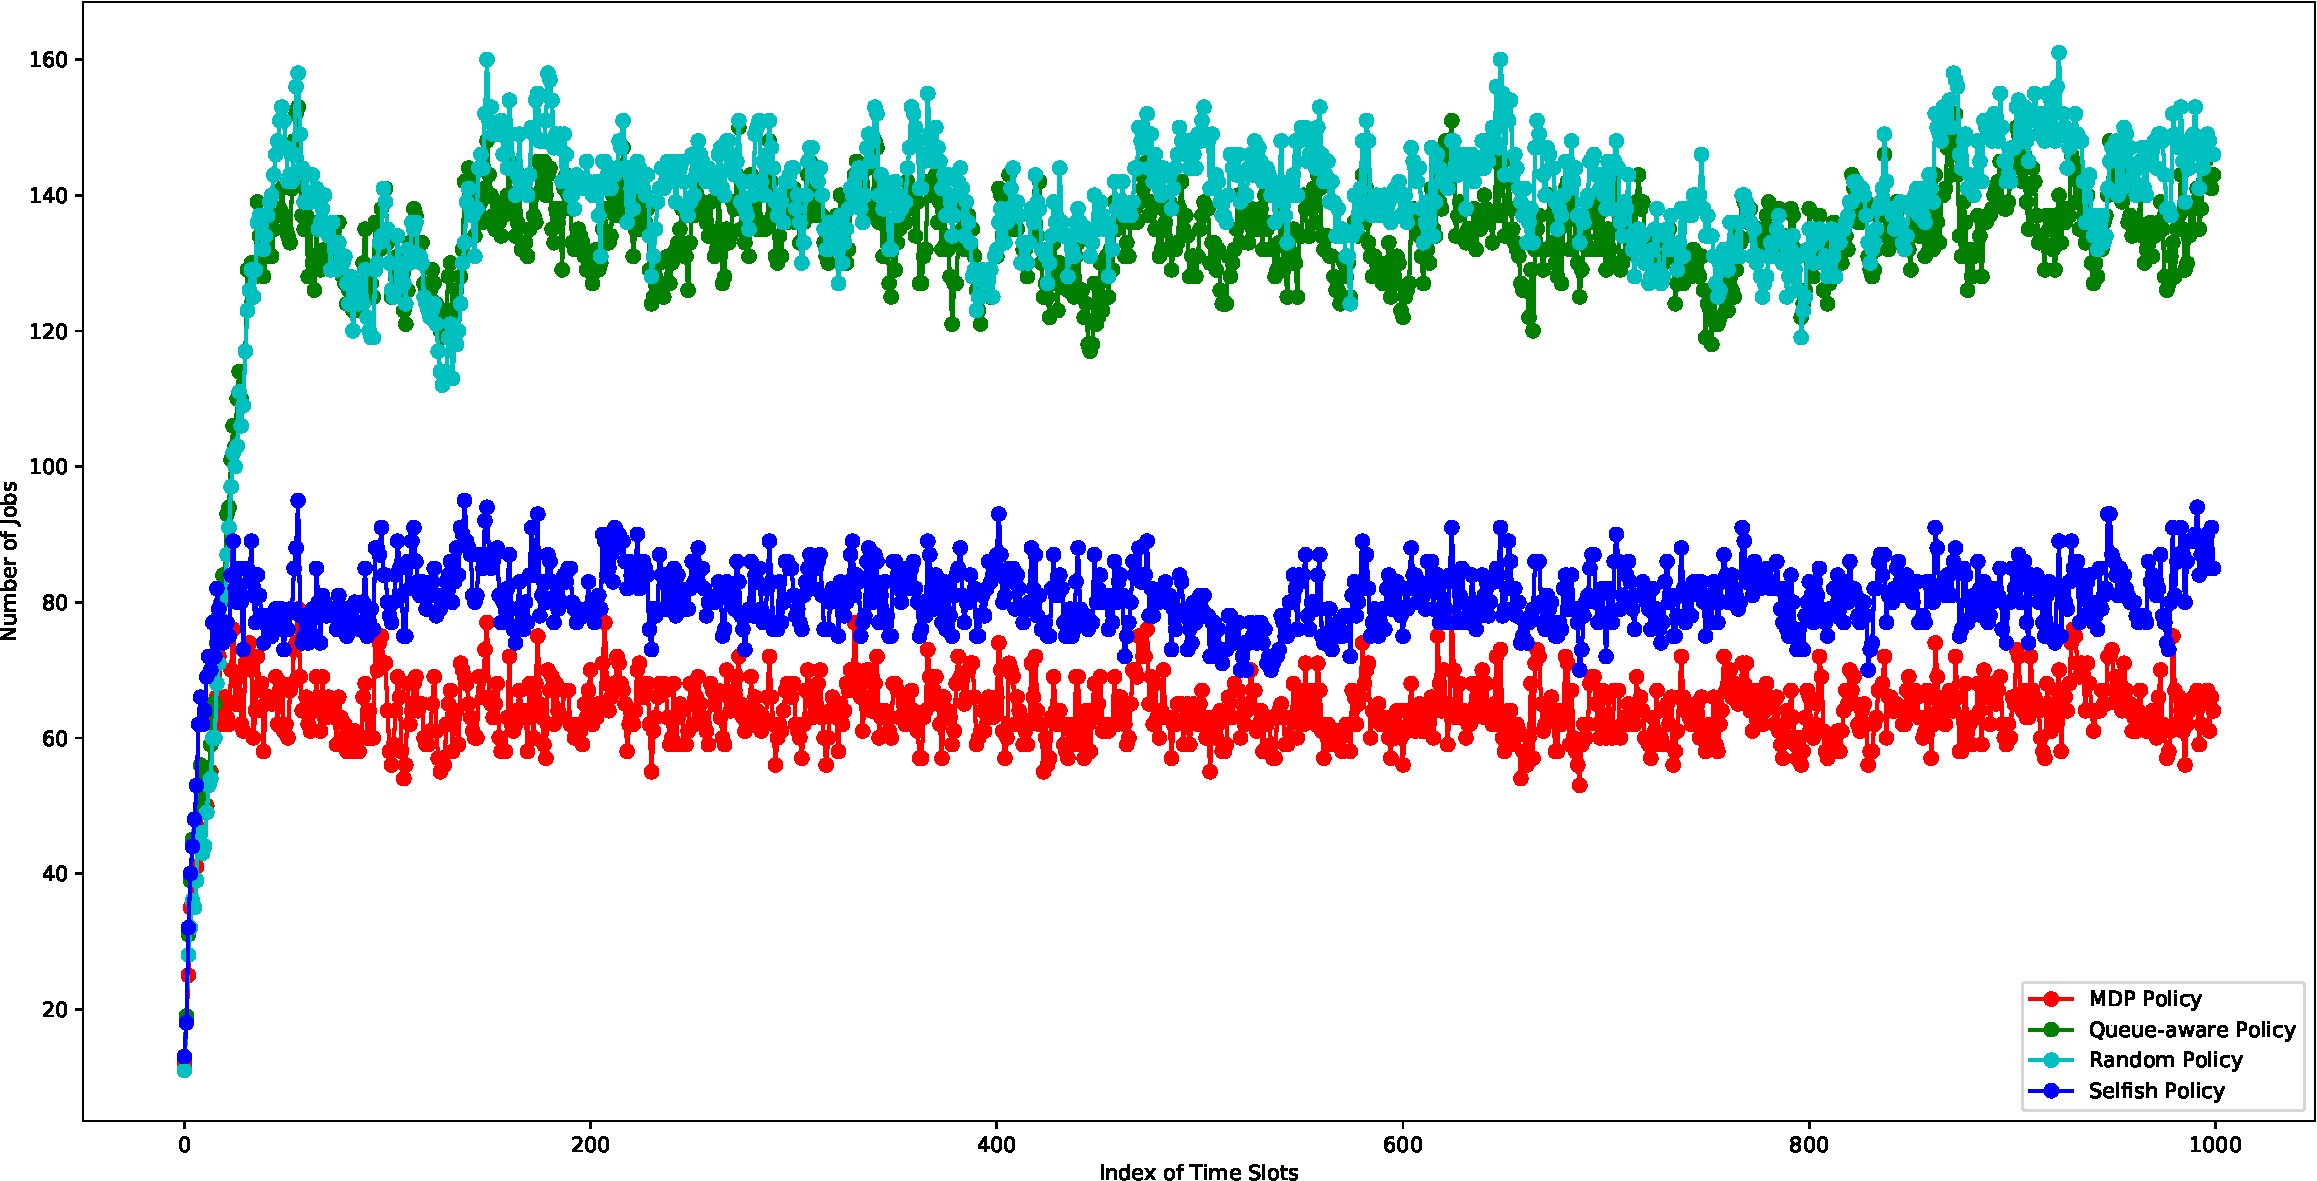
\includegraphics[width=0.80\textwidth]{48113-timeline-number.pdf}                           %
    \caption{Illustration of number of jobs on all the APs and edge servers over time.}     %
    \label{fig:general_timeline}                                                                %
\end{figure*}                                                                                   %
%-----------------------------------------------------------------------------------------------%

%NOTE: Benchmark Elaboration
\textbf{Benchmarks:}
We compare the proposed algorithm with other three heuristic algorithms which are listed as follows.
\begin{itemize}
    \item \textbf{Random Dispatching Policy}:
            for each job type, randomly choose the dispatching edge server in each time slot; 
    \item \textbf{Selfish Algorithm}:
            for each job type, always choose the edge server with the minimum expected uploading time, plus the expected processing time;
    \item \textbf{Queue-aware Selfish Algorithm}:
            for each job type, always choose the edge server with the minimum expected uploading time, plus the expected processing time and queueing time based on the observation of outdated queue states.
\end{itemize}
Specifically, we choose the \emph{Local Selfish Algorithm} which is state-invariant as the initial fixed policy for our proposed algorithm.
The explicit definition is given as follows.
\begin{policy}[Selfish Policy]
    \begin{align}
        \Baseline &\define \Brace{ \Pi_{k}\define\set{\pi_{k,j}|\forall j\in\jSpace} |\forall k\in\apSet },
    \end{align}
    where $\pi_{k,j} \define \arg\min_{m\in\esSet_{k}} u_{k,m,j} + c_{m,j}$.
\end{policy}

%NOTE: Basic Performance
Here we measure some basic metrics concerning in edge computing system, compared with different algorithms.
Average Cost v.s. Algorithms, Fig.\ref{fig:bar_plot}(a);
Average JCT (job completion time) v.s. Algorithms, Fig.\ref{fig:bar_plot}(b);
Average Departure Rate (throughput) v.s. Algorithms, Fig.\ref{fig:bar_plot}(c).

%-----------------------------------------------------------------------%
\begin{figure}[h]                                                       %
    \centering                                                          %
    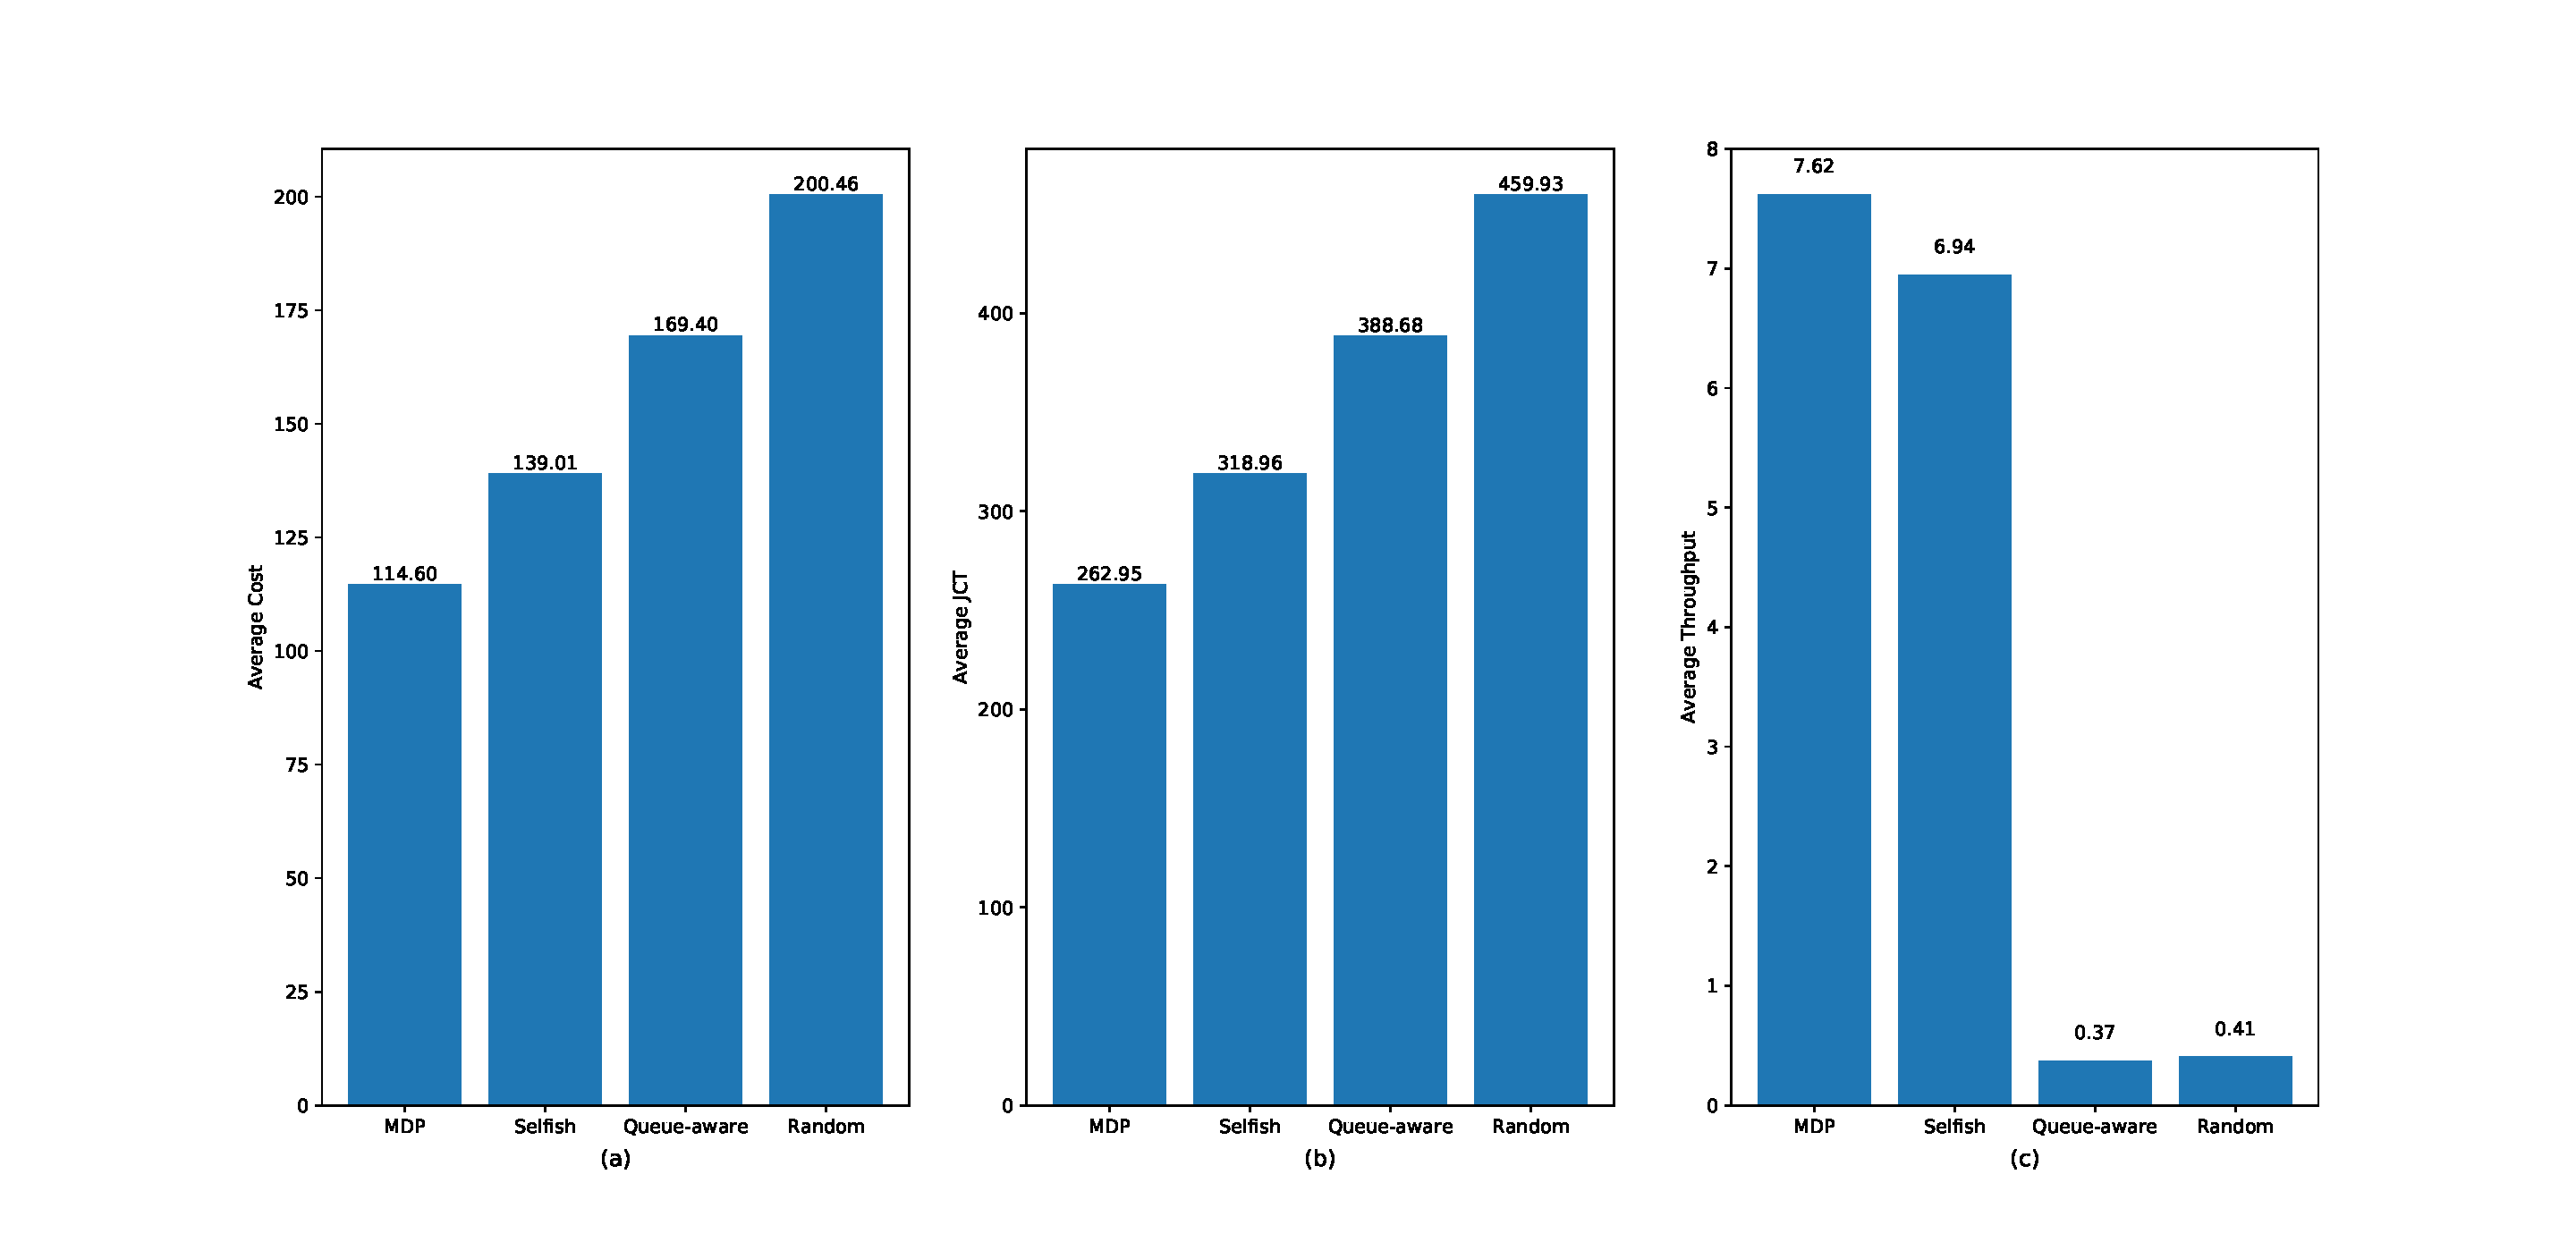
\includegraphics[width=0.45\textwidth]{48113-bar-graph.pdf}         %
    \caption{Illustration of performance metrics comparison with benchmarks.}
    \label{fig:bar_plot}                                                %
\end{figure}                                                            %
%-----------------------------------------------------------------------%

%NOTE: Insight Analysis
Specifically, 
our proposed algorithm is better than compared algorithms all the time;
CDF graph of Cost (with different benchmarks).
% CDF graph of JCT (with different algorithms).
%----------------------------------------------------------------------------------------%
\subsection{Performance Analysis}
\label{subsec:advance}
\blindtext

%FIXME: replace the graphs
%-----------------------------------------------------------------------------------------------%
\begin{figure*}[ht!]                                                                            %
    \centering                                                                                  %
    \begin{tabular}{ccc}                                                                        %
        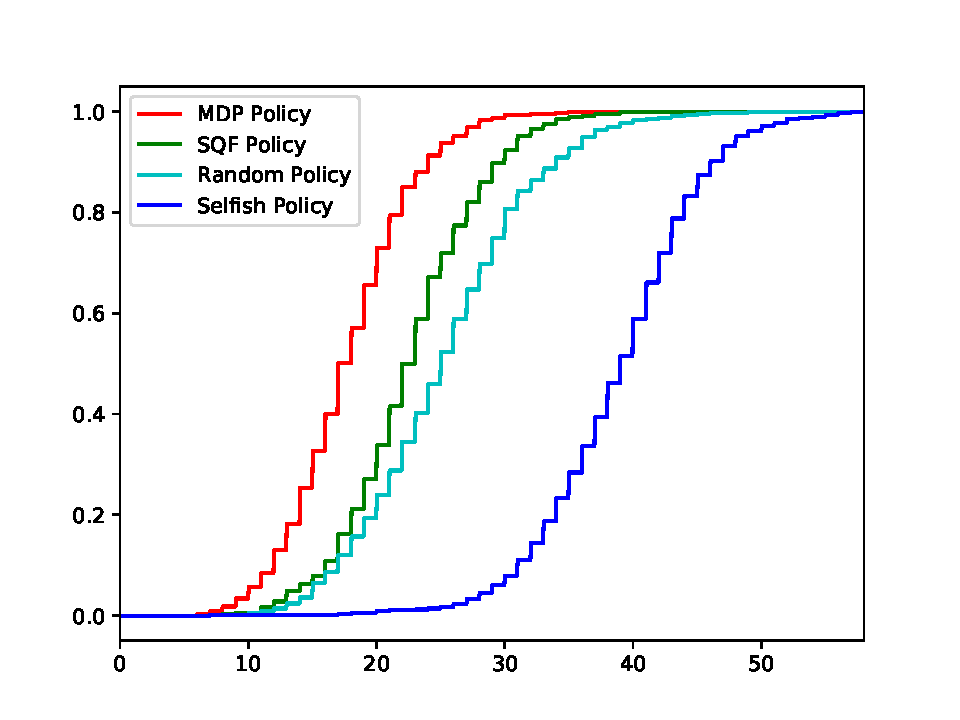
\includegraphics[width=0.30\textwidth]{images/535_LowPressure_NoDelay.pdf}&             %
        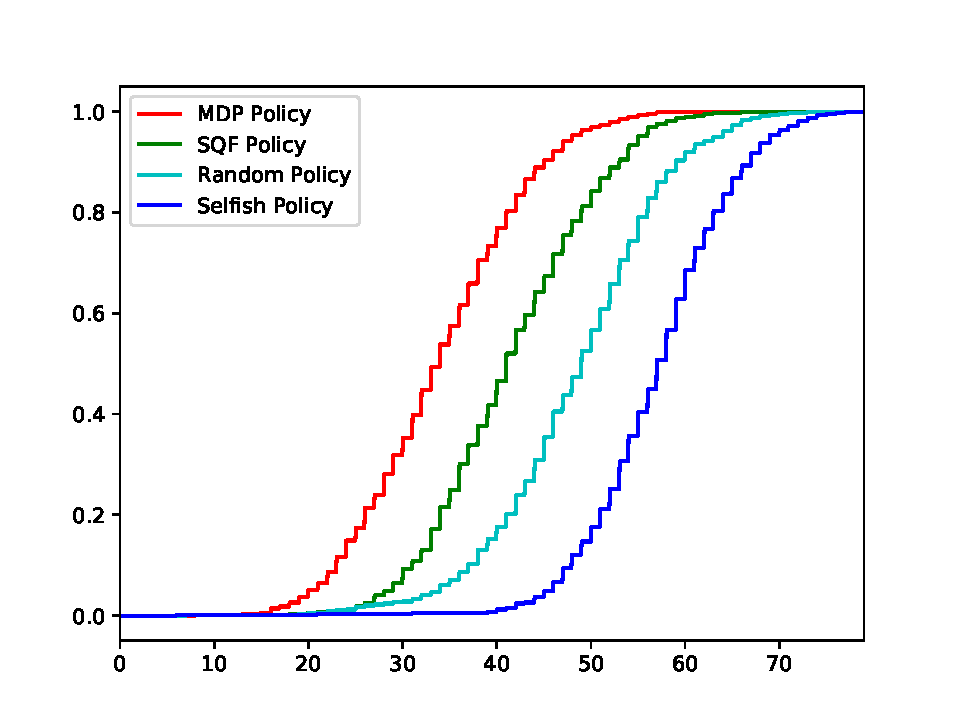
\includegraphics[width=0.30\textwidth]{images/535_LowPressure_LargeDelay_cdf.pdf}&      %
        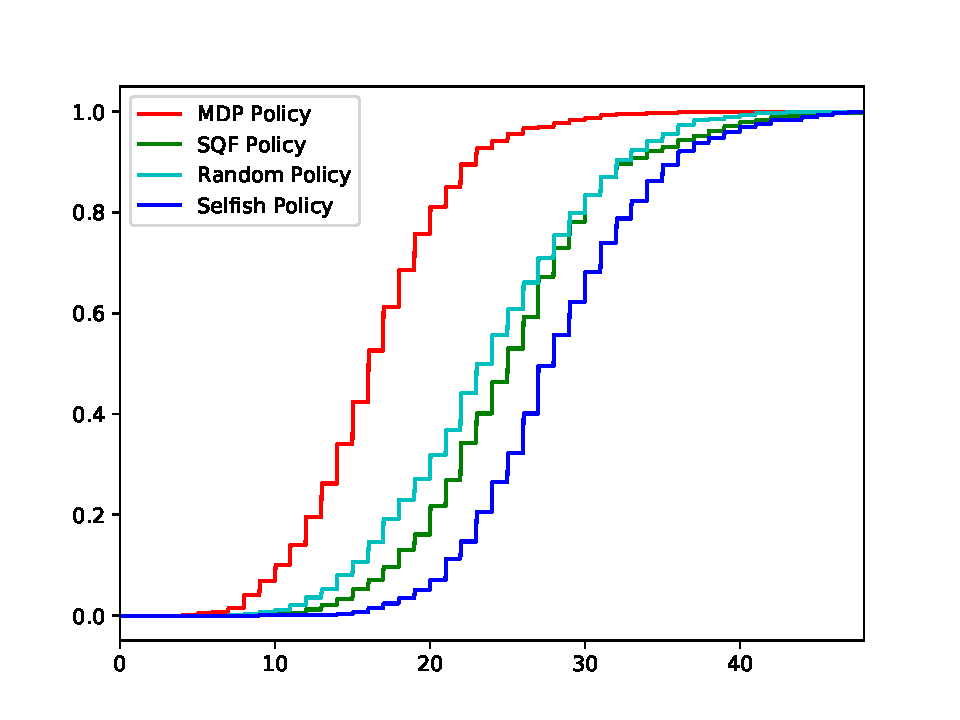
\includegraphics[width=0.30\textwidth]{images/535_LowPressure_FullDelay.pdf}            %
        \\                                                                                      %
        {\small (a) No \brlatency} &                                                            %
        {\small (b) Large \brlatency} &                                                         %
        {\small (c) Whole-interval \brlatency}                                                  %
    \end{tabular}                                                                               %
    \caption{Evaluation of Information Staleness Impact on Algorithm Robustness.}               %
    \label{fig:ss_delay}                                                                        %
\end{figure*}                                                                                   %
%-----------------------------------------------------------------------------------------------%

%-------------------------------------------------------------------%
\begin{figure}[hbt]                                                 %
    \centering                                                      %
    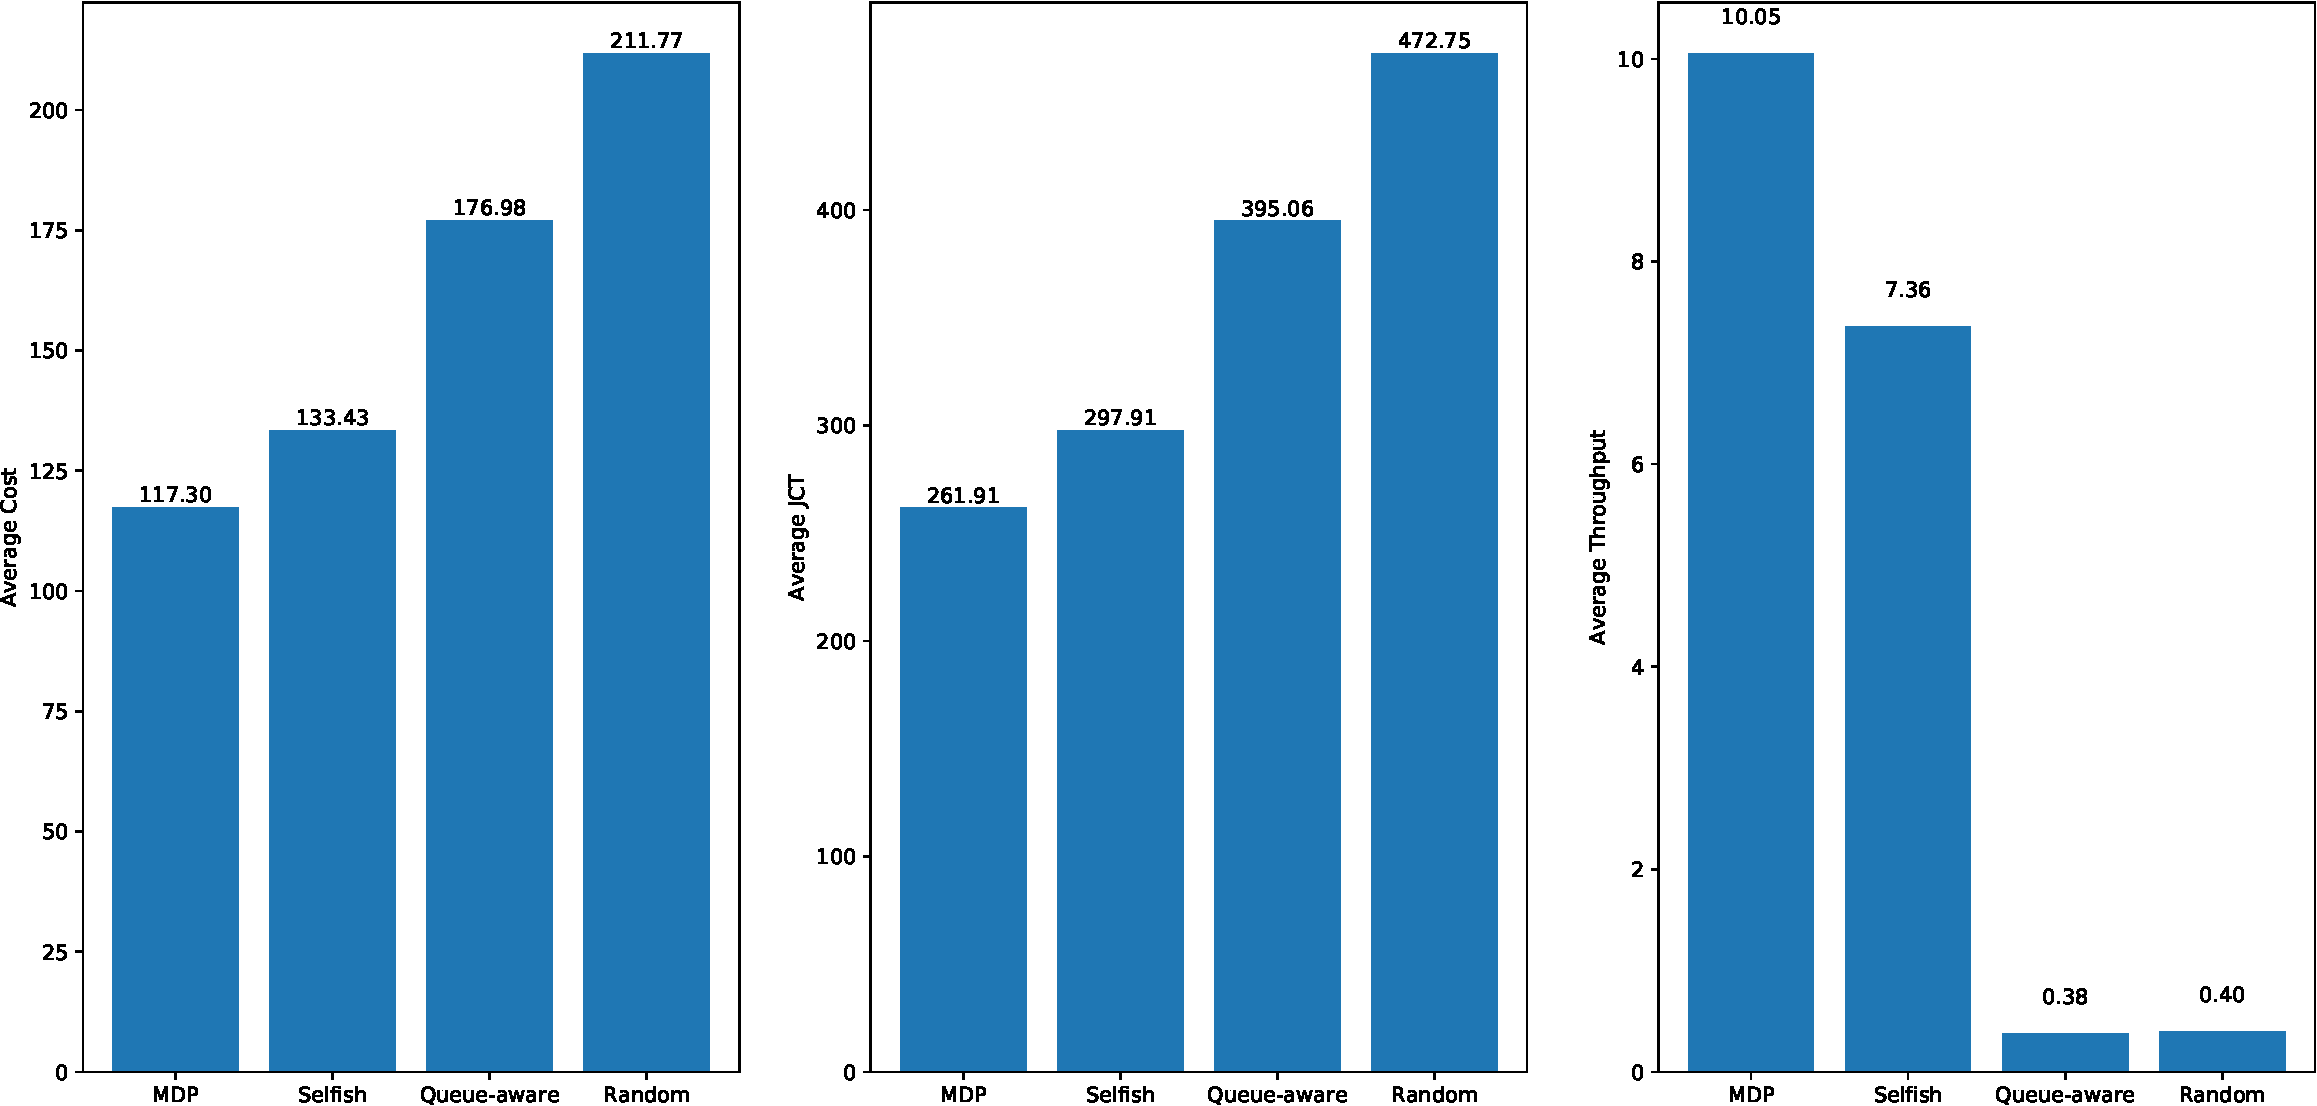
\includegraphics[width=0.45\textwidth]{bar_graph.pdf}           %
    \caption{}                                              %
    \label{fig:ss_scale}                                            %
\end{figure}                                                        %
%-------------------------------------------------------------------%

%-------------------------------------------------------------------%
\begin{figure}[hbt]                                                 %
    \centering                                                      %
    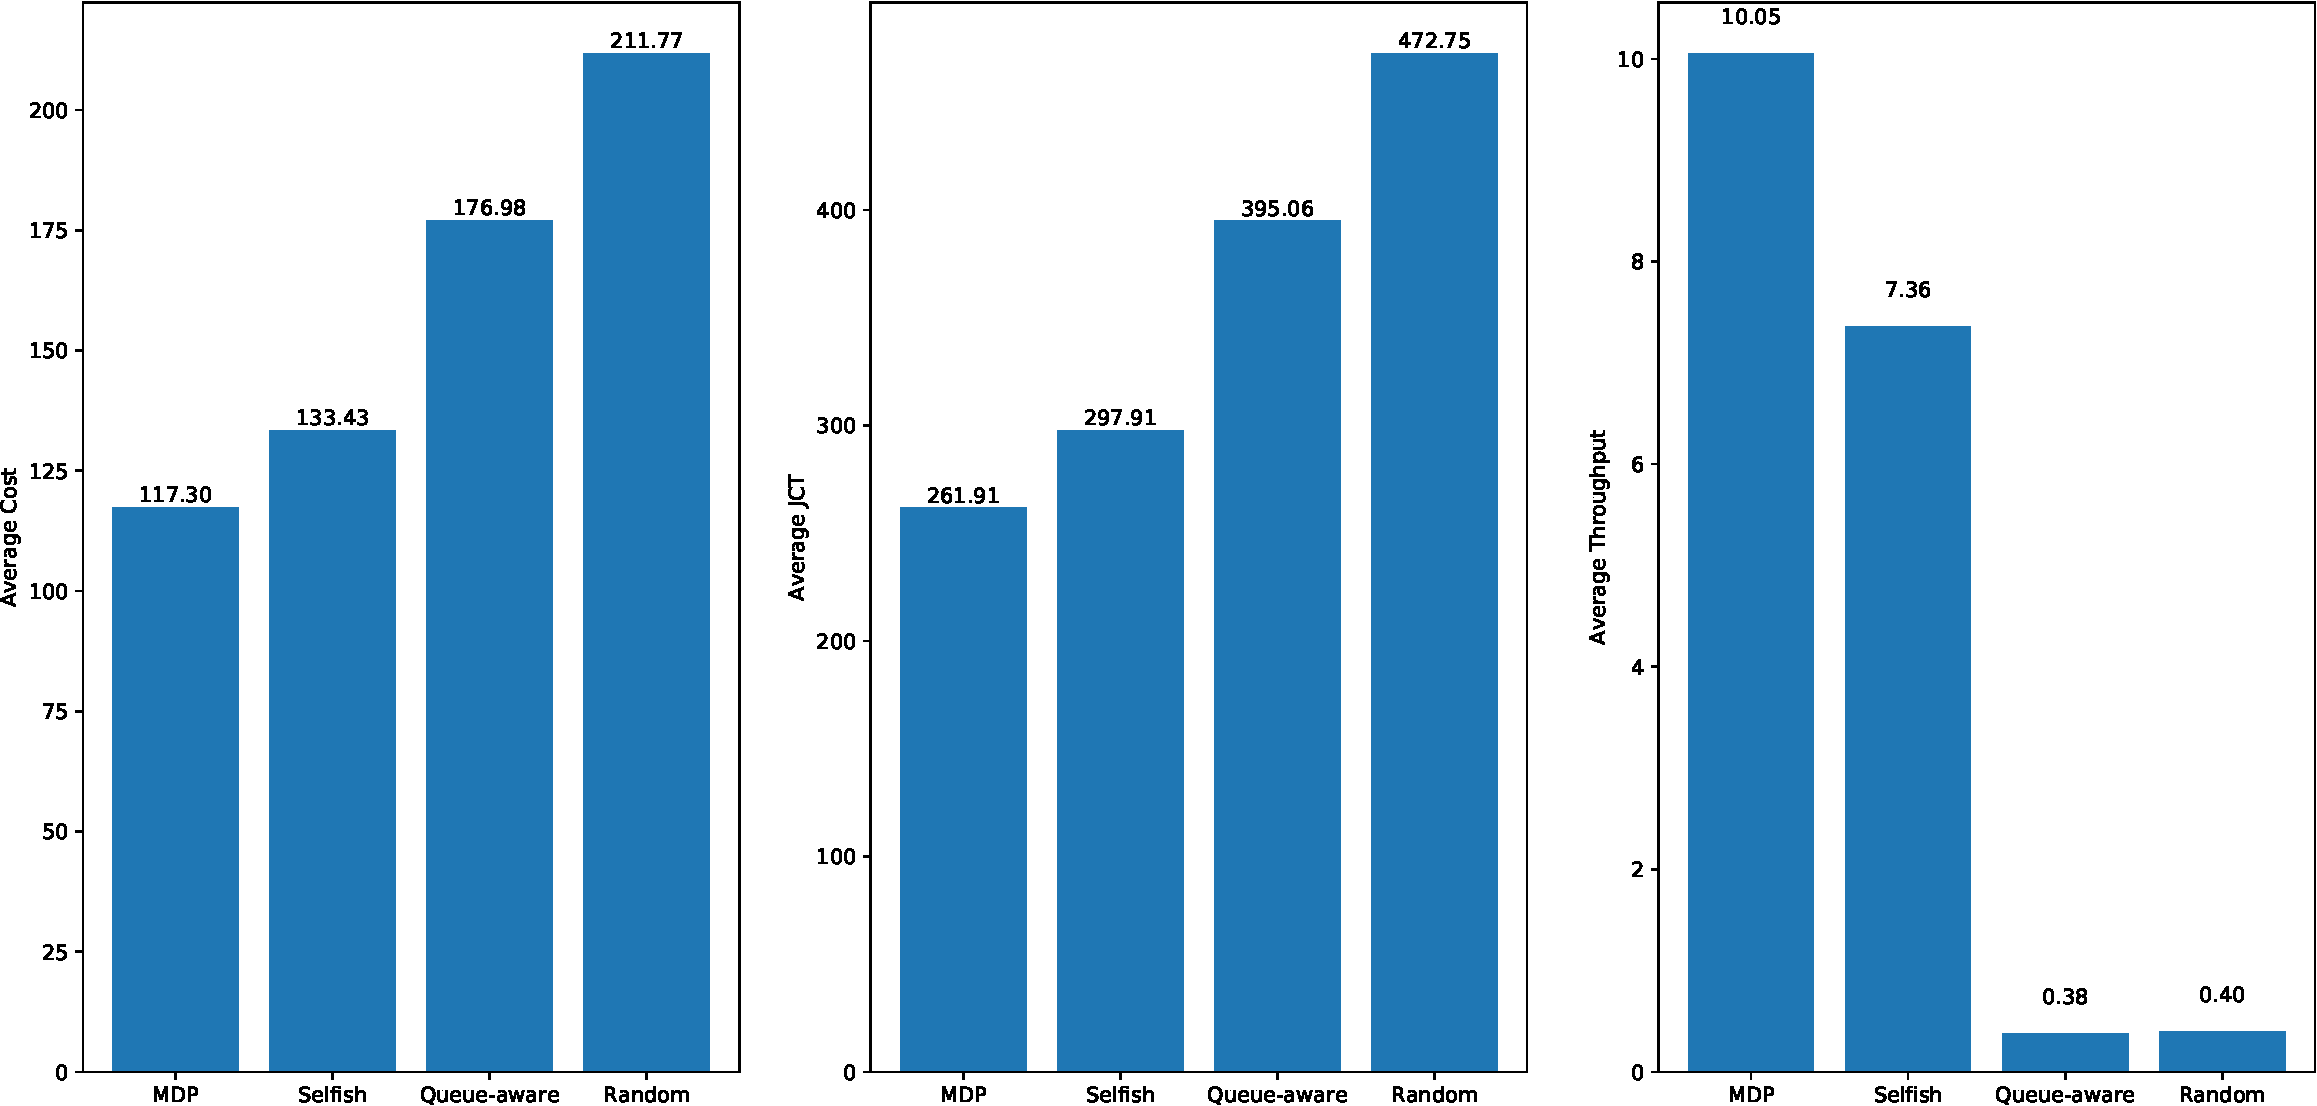
\includegraphics[width=0.45\textwidth]{bar_graph.pdf}           %
    \caption{Fake 02.}                                              %
    \label{fig:ss_dist}                                             %
\end{figure}                                                        %
%-------------------------------------------------------------------%

%-------------------------------------------------------------------%
\begin{figure}[hbt]                                                 %
    \centering                                                      %
    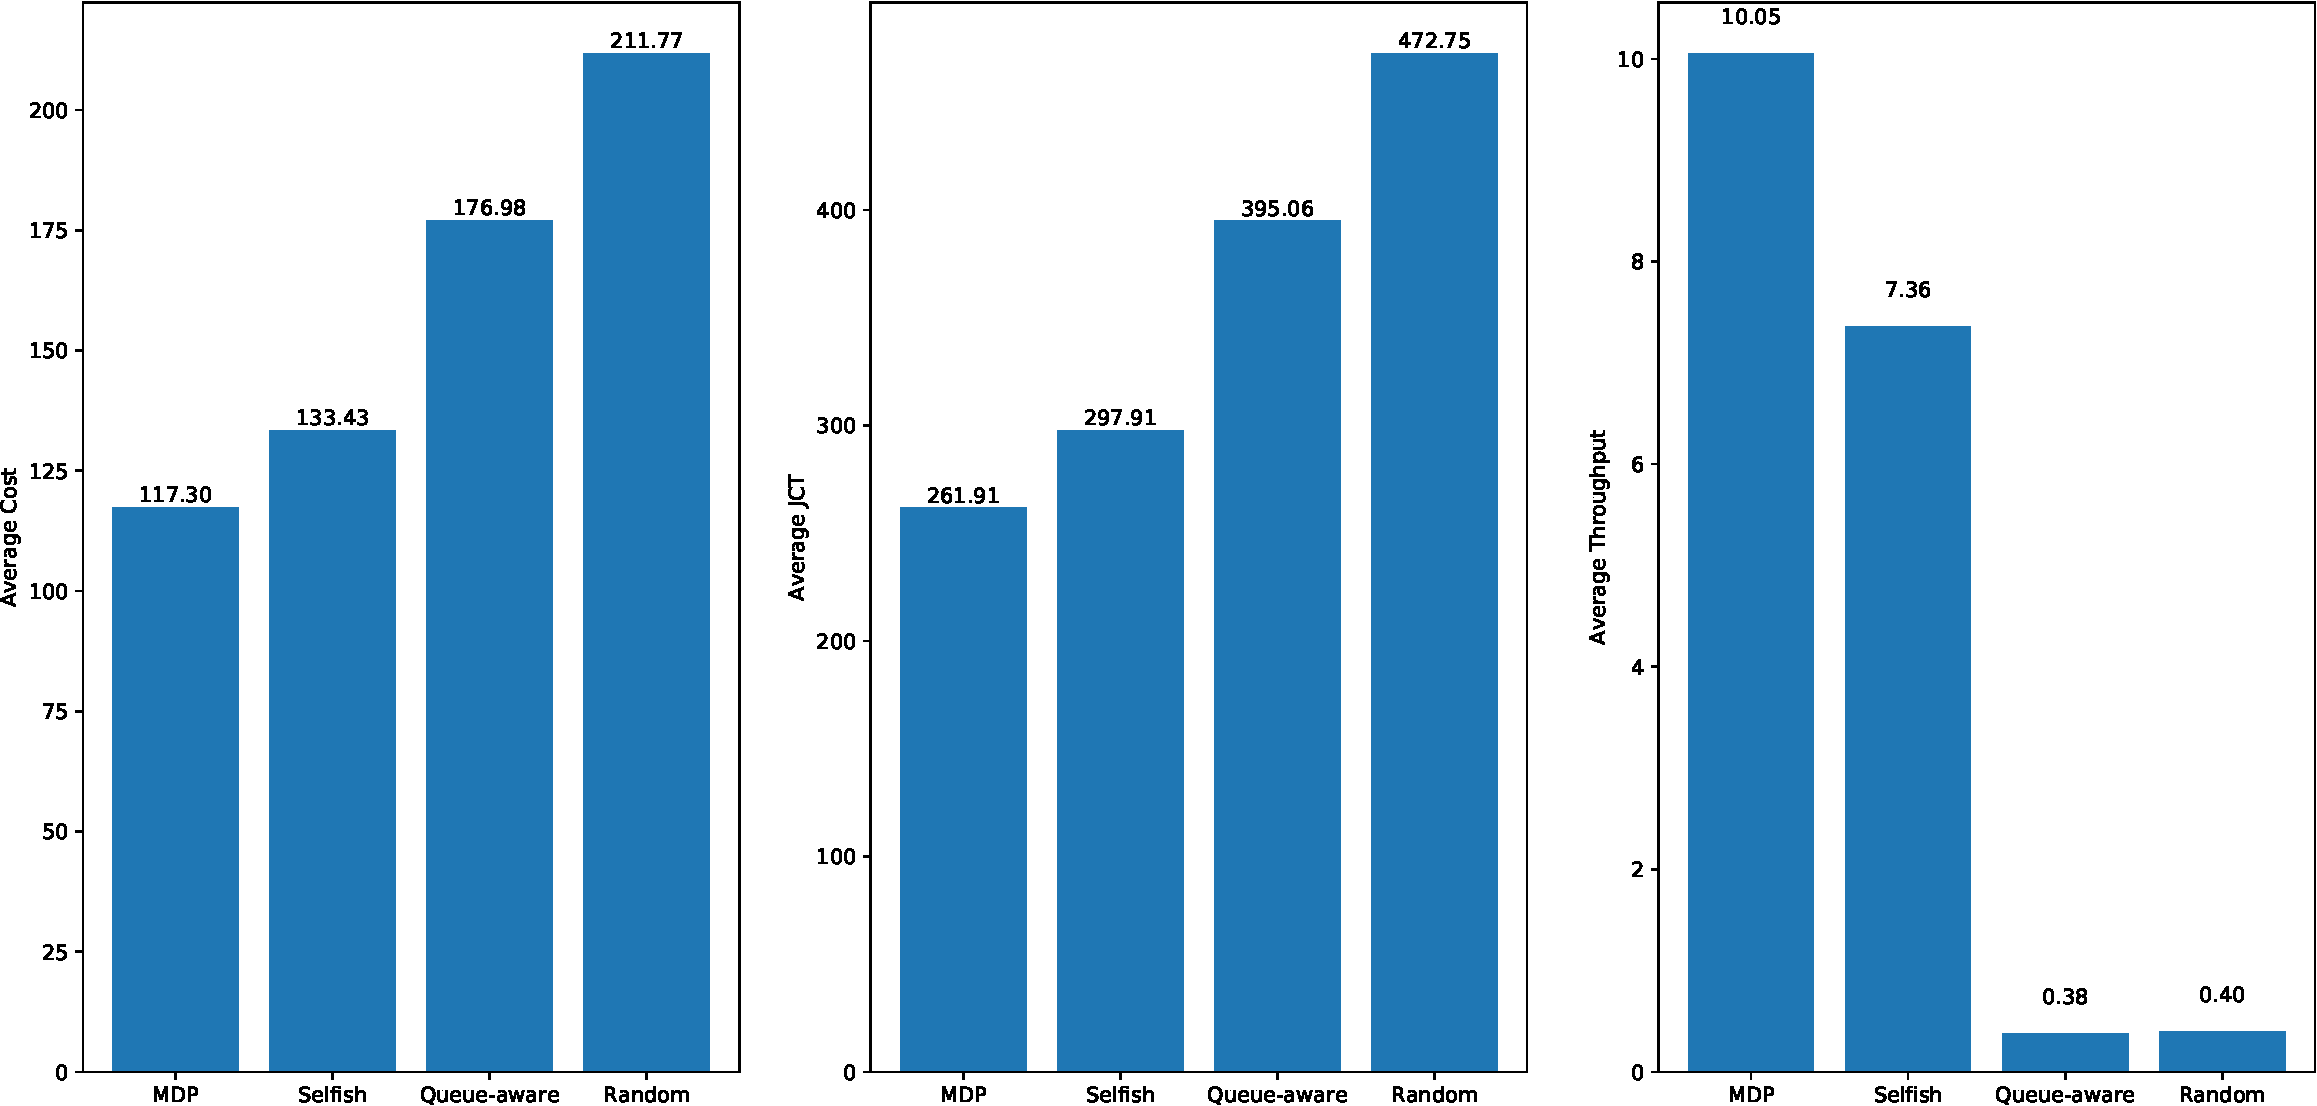
\includegraphics[width=0.45\textwidth]{bar_graph.pdf}           %
    \caption{}                                              %
    \label{fig:ss_scale}                                            %
\end{figure}                                                        %
%-------------------------------------------------------------------%

%NOTE: sensitivity study
\textbf{Compared with different \brlatency.}
The evaluation of staleness of \brlatency~is demonstrated in Fig.\ref{fig:ss_delay}.

\textbf{Uploading Time or Processing Time domains.}
The evaluation of distribution of is demonstrated in Fig.\ref{fig:ss_dist}.
\blindtext

\textbf{Number of APs.} %(a.k.a arrival rate)
The evaluation of scale of is demonstrated in Fig.\ref{fig:ss_scale}.
It's shown that on the left of the figure, the SQF algorithm would work better when the system is almost idle; on the right of the figure, SQF and random algorithm could not handle high rejection rate and thus the \emph{average throughput} decreases extremely. 

% \textbf{Different Penalty Factors.}
% CDF of \# of dropped jobs (over the queue limit); CDF of queue length;

%----------------------------------------------------------------------------------------%
